\chapter{Related work}
\section{Boundary attack}
\gls{ba} \cite{boundary_attack} is a decision-based adversarial attack. The basic intuition of \gls{ba} differs from traditional adversarial attacks. Unlike these traditional adversarial attacks, where the original image is moved through search space in order to become adversarial, \gls{ba} starts from an input that is already adversarial. This input is then moved closer to the original image, while staying adversarial.\\

The attack has to be initialized with an already adversarial input. Two different approaches can be taken depending on the attack setting. In the untargeted case, the input can be sampled from a maximum entropy distribution given the valid domain of this input. Samples that are not adversarial are rejected. In the case of a targeted attack, the input is a sample from the dataset that is classified as the target class by the model under attack.\\

\gls{ba} iteratively updates the adversarial image by performing a step orthogonal to the original image and a step towards this image. In iteration $k$, a perturbation $\eta_k$ is sampled from a Gaussian distribution. This perturbation is rescaled and added to the adversarial image. From this new position in search space, the step towards the original image is taken. This way the path of the attack follows the decision boundary, hence the name of the attack. The intuition of the \gls{ba} is shown in Figure~\ref{fig:boundary_attack_intuition}.\\

The step sizes are adjusted according to local geometry of the boundary. The orthogonal step size $\delta$ is adjusted so that approximately half of the orthogonal perturbations is still adversarial. This approach is based on trust region methods \cite{trm}. The step size towards the original image $\epsilon$ is adjusted using the same principle, but here a user specified threshold is used. The decision boundary tends to become flatter, the closer to the original image the attack gets. Therefore the algorithm converges when $\epsilon$ converges to zero.\\

Biased boundary\\

\begin{figure}
\centering
\tikzset{every picture/.style={line width=0.75pt}} %set default line width to 0.75pt        
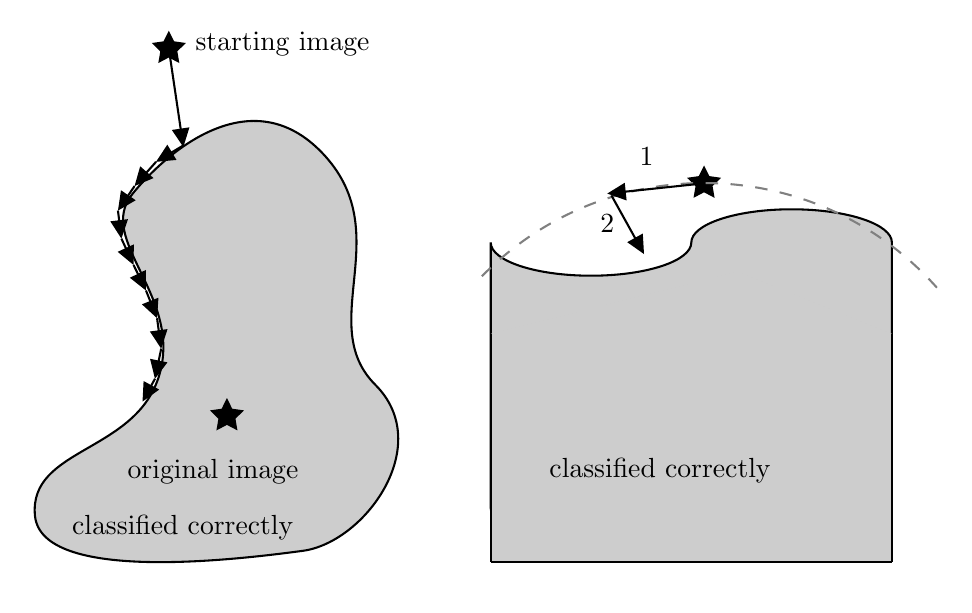
\begin{tikzpicture}[x=0.75pt,y=0.75pt,yscale=-1,xscale=1]
%uncomment if require: \path (0,300); %set diagram left start at 0, and has height of 300

%Shape: Polygon Curved [id:ds7418598759978794] 
\draw  [fill={rgb, 255:red, 155; green, 155; blue, 155 }  ,fill opacity=0.5 ] (77.12,92.56) .. controls (95.12,70.56) and (136.12,36.56) .. (170.12,74.56) .. controls (204.12,112.56) and (165.12,155.56) .. (194.12,184.56) .. controls (223.12,213.56) and (189.12,260.56) .. (159.12,264.56) .. controls (129.12,268.56) and (33.12,280.56) .. (30.12,247.56) .. controls (27.12,214.56) and (79.12,217.56) .. (90.12,179.56) .. controls (101.12,141.56) and (59.12,114.56) .. (77.12,92.56) -- cycle ;
%Shape: Star [id:dp3640249127076376] 
\draw  [fill={rgb, 255:red, 0; green, 0; blue, 0 }  ,fill opacity=1 ] (122.62,192.06) -- (124.83,196.53) -- (129.76,197.24) -- (126.19,200.72) -- (127.03,205.63) -- (122.62,203.31) -- (118.22,205.63) -- (119.06,200.72) -- (115.49,197.24) -- (120.42,196.53) -- cycle ;
%Shape: Star [id:dp11559629314794817] 
\draw  [fill={rgb, 255:red, 0; green, 0; blue, 0 }  ,fill opacity=1 ] (94.62,15.06) -- (96.83,19.53) -- (101.76,20.24) -- (98.19,23.72) -- (99.03,28.63) -- (94.62,26.31) -- (90.22,28.63) -- (91.06,23.72) -- (87.49,20.24) -- (92.42,19.53) -- cycle ;
%Straight Lines [id:da5485453367188926] 
\draw    (94.62,22.56) -- (101.19,67.01) ;
\draw [shift={(101.62,69.98)}, rotate = 261.6] [fill={rgb, 255:red, 0; green, 0; blue, 0 }  ][line width=0.08]  [draw opacity=0] (8.93,-4.29) -- (0,0) -- (8.93,4.29) -- cycle    ;
%Straight Lines [id:da4671198010612545] 
\draw    (101.79,69.14) -- (91.03,75.6) ;
\draw [shift={(88.46,77.14)}, rotate = 329.04] [fill={rgb, 255:red, 0; green, 0; blue, 0 }  ][line width=0.08]  [draw opacity=0] (8.93,-4.29) -- (0,0) -- (8.93,4.29) -- cycle    ;
%Straight Lines [id:da7587598831272953] 
\draw    (88.46,77.14) -- (80.11,86.56) ;
\draw [shift={(78.12,88.81)}, rotate = 311.53] [fill={rgb, 255:red, 0; green, 0; blue, 0 }  ][line width=0.08]  [draw opacity=0] (8.93,-4.29) -- (0,0) -- (8.93,4.29) -- cycle    ;
%Straight Lines [id:da4110511376379753] 
\draw    (78.12,88.81) -- (71.8,98.16) ;
\draw [shift={(70.12,100.64)}, rotate = 304.06] [fill={rgb, 255:red, 0; green, 0; blue, 0 }  ][line width=0.08]  [draw opacity=0] (8.93,-4.29) -- (0,0) -- (8.93,4.29) -- cycle    ;
%Straight Lines [id:da1003086206787116] 
\draw    (70.12,100.64) -- (71.42,111.17) ;
\draw [shift={(71.79,114.14)}, rotate = 262.96] [fill={rgb, 255:red, 0; green, 0; blue, 0 }  ][line width=0.08]  [draw opacity=0] (8.93,-4.29) -- (0,0) -- (8.93,4.29) -- cycle    ;
%Straight Lines [id:da8276465700326683] 
\draw    (71.79,114.14) -- (76.37,124.08) ;
\draw [shift={(77.62,126.81)}, rotate = 245.27] [fill={rgb, 255:red, 0; green, 0; blue, 0 }  ][line width=0.08]  [draw opacity=0] (8.93,-4.29) -- (0,0) -- (8.93,4.29) -- cycle    ;
%Straight Lines [id:da3087971830978391] 
\draw    (77.62,126.81) -- (82.31,136.45) ;
\draw [shift={(83.62,139.14)}, rotate = 244.06] [fill={rgb, 255:red, 0; green, 0; blue, 0 }  ][line width=0.08]  [draw opacity=0] (8.93,-4.29) -- (0,0) -- (8.93,4.29) -- cycle    ;
%Straight Lines [id:da0022003187287755743] 
\draw    (83.62,139.14) -- (87.84,149.69) ;
\draw [shift={(88.96,152.48)}, rotate = 248.2] [fill={rgb, 255:red, 0; green, 0; blue, 0 }  ][line width=0.08]  [draw opacity=0] (8.93,-4.29) -- (0,0) -- (8.93,4.29) -- cycle    ;
%Straight Lines [id:da534724447641469] 
\draw    (88.96,152.48) -- (90.55,164.17) ;
\draw [shift={(90.96,167.14)}, rotate = 262.23] [fill={rgb, 255:red, 0; green, 0; blue, 0 }  ][line width=0.08]  [draw opacity=0] (8.93,-4.29) -- (0,0) -- (8.93,4.29) -- cycle    ;
%Straight Lines [id:da922850059483852] 
\draw    (90.96,167.14) -- (88.57,178.7) ;
\draw [shift={(87.96,181.64)}, rotate = 281.69] [fill={rgb, 255:red, 0; green, 0; blue, 0 }  ][line width=0.08]  [draw opacity=0] (8.93,-4.29) -- (0,0) -- (8.93,4.29) -- cycle    ;
%Straight Lines [id:da8803758051874986] 
\draw    (87.96,181.64) -- (83.39,190.01) ;
\draw [shift={(81.96,192.64)}, rotate = 298.61] [fill={rgb, 255:red, 0; green, 0; blue, 0 }  ][line width=0.08]  [draw opacity=0] (8.93,-4.29) -- (0,0) -- (8.93,4.29) -- cycle    ;

%Flowchart: Punched Tape [id:dp32393516464120875] 
\draw  [color={rgb, 255:red, 0; green, 0; blue, 0 }  ,draw opacity=1 ][fill={rgb, 255:red, 155; green, 155; blue, 155 }  ,fill opacity=0.5 ] (249.71,116) .. controls (249.71,124.84) and (271.35,132) .. (298.04,132) .. controls (324.72,132) and (346.36,124.84) .. (346.36,116) .. controls (346.36,107.16) and (367.99,100) .. (394.68,100) .. controls (421.37,100) and (443,107.16) .. (443,116) -- (443,244) .. controls (443,235.16) and (421.37,228) .. (394.68,228) .. controls (367.99,228) and (346.36,235.16) .. (346.36,244) .. controls (346.36,252.84) and (324.72,260) .. (298.04,260) .. controls (271.35,260) and (249.71,252.84) .. (249.71,244) -- cycle ;
%Shape: Polygon [id:ds9050991390362941] 
\draw  [draw opacity=0][fill={rgb, 255:red, 205; green, 205; blue, 205 }  ,fill opacity=1 ] (368.66,130) -- (443,160) -- (443,270) -- (249.71,270) -- (249.71,160) -- cycle ;
%Straight Lines [id:da7257665454280118] 
\draw    (249.71,160) -- (249.71,270) ;
%Straight Lines [id:da16137593574333753] 
\draw    (443,270) -- (249.71,270) ;
%Straight Lines [id:da4234135136369108] 
\draw    (443,270) -- (443,160) ;

%Shape: Star [id:dp044247029438336805] 
\draw  [fill={rgb, 255:red, 0; green, 0; blue, 0 }  ,fill opacity=1 ] (352.5,80) -- (354.7,84.47) -- (359.63,85.18) -- (356.07,88.66) -- (356.91,93.57) -- (352.5,91.25) -- (348.09,93.57) -- (348.93,88.66) -- (345.37,85.18) -- (350.3,84.47) -- cycle ;
%Shape: Arc [id:dp333916759593228] 
\draw  [draw opacity=0][dash pattern={on 4.5pt off 4.5pt}] (245.44,132.3) .. controls (272.66,104.56) and (310.57,87.36) .. (352.5,87.36) .. controls (398.82,87.36) and (440.23,108.35) .. (467.75,141.34) -- (352.5,237.36) -- cycle ; \draw  [color={rgb, 255:red, 128; green, 128; blue, 128 }  ,draw opacity=1 ][dash pattern={on 4.5pt off 4.5pt}] (245.44,132.3) .. controls (272.66,104.56) and (310.57,87.36) .. (352.5,87.36) .. controls (398.82,87.36) and (440.23,108.35) .. (467.75,141.34) ;
%Straight Lines [id:da9368796655989884] 
\draw    (352.5,87.5) -- (308.84,92.11) ;
\draw [shift={(305.86,92.43)}, rotate = 353.97] [fill={rgb, 255:red, 0; green, 0; blue, 0 }  ][line width=0.08]  [draw opacity=0] (8.93,-4.29) -- (0,0) -- (8.93,4.29) -- cycle    ;
%Straight Lines [id:da5017346853785729] 
\draw    (307.86,93.29) -- (322.11,118.95) ;
\draw [shift={(323.57,121.57)}, rotate = 240.95] [fill={rgb, 255:red, 0; green, 0; blue, 0 }  ][line width=0.08]  [draw opacity=0] (8.93,-4.29) -- (0,0) -- (8.93,4.29) -- cycle    ;

% Text Node
\draw (120.12,226.56) node   [align=left] {\begin{minipage}[lt]{68pt}\setlength\topsep{0pt}
original image
\end{minipage}};
% Text Node
\draw (342.21,225.86) node   [align=left] {\begin{minipage}[lt]{96.27pt}\setlength\topsep{0pt}
classified correctly
\end{minipage}};
% Text Node
\draw (112.21,253.14) node   [align=left] {\begin{minipage}[lt]{96.27pt}\setlength\topsep{0pt}
classified correctly
\end{minipage}};
% Text Node
\draw (320,69) node [anchor=north west][inner sep=0.75pt]   [align=left] {1};
% Text Node
\draw (301,101) node [anchor=north west][inner sep=0.75pt]   [align=left] {2};
% Text Node
\draw (106,13) node [anchor=north west][inner sep=0.75pt]   [align=left] {starting image};


\end{tikzpicture}
\caption[Intuition of the Boundary Attack]{Intuition behind the Boundary Attack. On the left the path of the attack is shown. It follows the decision boundary of the class of the original image. Each arrow represents one iteration of the attack. On the right, the two different steps of each iteration can be seen. The first step is orthogonal to the original image (dashed circle) and the second step is towards the original image.}
\label{fig:boundary_attack_intuition}
\end{figure}